% =====================================================================
% Multi-Agent Academic Helpdesk for IIT Jodhpur -- Project Report
% Compile with:  pdflatex REPORT.tex  (twice, for the table of contents)
% Self-contained: all figures are drawn in TikZ/pgfplots; no external files are needed.
% =====================================================================
\documentclass[10pt,a4paper]{article}

\usepackage[utf8]{inputenc}
\usepackage[T1]{fontenc}
\usepackage{lmodern}
\usepackage[margin=2.0cm]{geometry}
\usepackage{booktabs}
\usepackage{array}
\usepackage{tabularx}
\usepackage{longtable}
\usepackage{graphicx}
\usepackage{float}
\usepackage[font=small,labelfont=bf]{caption}
\usepackage{xcolor}
\usepackage{colortbl}
\usepackage{amssymb}
\definecolor{good}{HTML}{0CA30C}
\definecolor{warn}{HTML}{FAB219}
\definecolor{crit}{HTML}{D03B3B}
\definecolor{neutral}{HTML}{C3C2B7}
\usepackage{enumitem}
\usepackage{listings}
\usepackage{microtype}
\usepackage{tikz}
\usetikzlibrary{positioning,arrows.meta,shapes.misc,fit,calc}
\usepackage{pgfplots}
\pgfplotsset{compat=1.17}
\usepackage[colorlinks=true,linkcolor=blue!50!black,urlcolor=blue!50!black,citecolor=blue!50!black]{hyperref}

\setlist{itemsep=1pt,topsep=2pt}
\setlength{\parskip}{2pt}
\setlength{\parindent}{0pt}
\renewcommand{\arraystretch}{1.06}

% Identifiers and file names: underscores and braces are printed literally.
\newcommand{\code}[1]{\texttt{\detokenize{#1}}}

\lstset{
  basicstyle=\ttfamily\footnotesize,
  breaklines=true,
  frame=single,
  framerule=0.3pt,
  rulecolor=\color{black!30},
  columns=fullflexible,
  keepspaces=true
}

\newcolumntype{Y}{>{\raggedright\arraybackslash}X}

\begin{document}

% ---------------------------------------------------------------------
% Title page
% ---------------------------------------------------------------------
\begin{titlepage}
\centering
\vspace*{1.2cm}
{\large Indian Institute of Technology Jodhpur\par}
{\normalsize Course: Autonomous Systems \quad|\quad Semester VII, Academic Year 2026--27\par}
\vspace{2.2cm}
{\Huge\bfseries Multi-Agent Academic Helpdesk\\[4pt] for IIT Jodhpur\par}
\vspace{0.8cm}
{\Large Retrieval-augmented generation with deterministic tools\\ and evidence-driven refusal, built on Google ADK\par}
\vspace{2.2cm}
{\Large\bfseries Project Report\par}
\vspace{1.6cm}

\begin{tabular}{@{}ll@{}}
\toprule
\textbf{Name} & \textbf{Roll number}\\
\midrule
Jatin Purbia & B23CH1022\\
Anuj Trivedi & B23CH1006\\
Sharana Gouda Lakshetty & B23CH1042\\
\bottomrule
\end{tabular}

\vspace{1.6cm}
Repository: \url{https://github.com/Sharan4405/Academic-_Helpdesk_Agent}
\vfill
{\normalsize Academic Year 2026--27}
\end{titlepage}

% ---------------------------------------------------------------------
% Abstract
% ---------------------------------------------------------------------
\begin{abstract}
\noindent
We built a multi-agent academic helpdesk for IIT Jodhpur that answers questions on rules, curriculum, the timetable and course offerings, drafts (never sends) emails to instructors, and refuses and logs everything else. An orchestrator routes each question to a policy, schedule or email agent. Rules are answered by retrieval over 33 official documents (390 chunks); counts, slots and contacts come from deterministic CSV tools. The evaluation set has 30 questions in four categories. Without a chat model, the evidence given to the agent is right for 24 of 25 answerable questions, 15 of 16 evidence verdicts are correct, 48 tool assertions pass, and the expected document ranks first for 10 of 11 policy questions (MRR 0.918). Trimming prompts and tool definitions cut a turn from about 120~s to about 70~s on a rate-limited hosted model. The main trade-off is that scope refusal cannot be enforced by retrieval distance (the in-scope and out-of-scope ranges overlap by 0.142) and so depends on the prompt. Model-answer scoring was not completed; explicitly labelled single-point estimates are given instead. The key lesson is to inspect what the model is shown: two defects were in the evidence, not the model.
\end{abstract}

\noindent\textbf{Keywords:} retrieval-augmented generation; multi-agent systems; Google ADK; academic helpdesk; grounded citation; refusal; hybrid retrieval; evaluation.

\tableofcontents
\clearpage

% =====================================================================
\section{Introduction}
% =====================================================================
A student asking ``What is the attendance requirement to sit in the Major exam?'' faces documents that disagree. The 2019 and 2022 academic regulations describe one rule; a July 2024 circular supersedes it, stating that examination performance is no longer linked to attendance while attendance should still not fall below 75\%. A general-purpose chat model answers from memory and will state a plausible threshold with confidence; a keyword search returns the longer, older regulation first. Both give a fluent wrong answer, and neither can say ``I do not know'' for questions the documents never cover, such as dining options.

The hard part of this task is therefore not answering but \emph{not} answering: a helpful model will invent an attendance threshold, an instructor's email address, or a count of electives. The objectives of the system are:
\begin{enumerate}
  \item Answer rules, regulations, calendar and curriculum questions from official documents, citing the document and page.
  \item Answer slot, room and course-count questions from structured data by code, so that numbers cannot drift between runs.
  \item Draft emails to the correct instructor for sick leave, make-up examinations and attendance condonation, without sending them.
  \item Refuse out-of-scope questions, and log each refusal for a human.
  \item Prefer the latest circular over the regulation it supersedes.
  \item Run within the constraints of a student laptop and a free hosted-model tier.
\end{enumerate}
Section~\ref{sec:req} states requirements; Sections~\ref{sec:data}--\ref{sec:pipeline} describe data, architecture and the retrieval pipeline; Section~\ref{sec:impl} covers implementation; Sections~\ref{sec:evalmethod}--\ref{sec:analysis} present the evaluation, results and analysis; Sections~\ref{sec:limits}--\ref{sec:future} give limitations and recommendations; Section~\ref{sec:repro} lists reproduction commands.

% =====================================================================
\section{Requirements and Scope}\label{sec:req}
% =====================================================================
\textbf{In scope.}
\begin{itemize}
  \item \emph{Rules and regulations:} attendance, examinations, make-up policy, withdrawal, probation, grading, fees, forms.
  \item \emph{Curriculum and calendar:} credit definitions, programme structures, dates in the academic calendar.
  \item \emph{Timetable and offerings:} slot of a course, its days and times, room, instructor, counts of courses by department and level, slot clashes.
  \item \emph{Email drafting:} instructor lookup and a draft for sick leave, make-up examination or attendance condonation.
\end{itemize}
\textbf{Out of scope.} Dining, hostel life, transport and reaching the campus, weather, sports facilities, and any question about a specific student's own record. Success here means the system says ``I do not know'', does not guess, and appends the question to a log with status \code{pending_human_review}.

\begin{table}[H]
\centering\small
\caption{Representative questions per category (full set in Appendix~A).}\label{tab:examples}
\begin{tabularx}{\textwidth}{@{}lY@{}}
\toprule
\textbf{Category} & \textbf{Example}\\
\midrule
Rules and calendar & What is the attendance requirement to sit in the Major exam? (Q01)\\
Timetable and offerings & How many 400 level electives have been floated by the Humanities department in this semester? (Q13)\\
Email & Write an email to the course instructor of CSL7570 that I need leave for 2 days. (Q21)\\
Out of scope & What are the available dining options on the campus? (Q26)\\
\bottomrule
\end{tabularx}
\end{table}

% =====================================================================
\section{Data Collection and Knowledge Sources}\label{sec:data}
% =====================================================================
\textbf{Documents.} The knowledge base is 33 official IIT Jodhpur documents, embedded as 390 chunks. The collection manifest (\code{data1/manifest_source.csv}) records, for 29 of them, the fields \code{doc_id}, \code{title}, \code{category}, \code{file}, \code{source_url}, \code{fetched_on}, \code{pages} and \code{sha256}: 25 were fetched from \code{iitj.ac.in} and 4 from \code{intranet.iitj.ac.in}, totalling 382 pages. Four indexed documents have no manifest row, so their source addresses are not recorded: \code{ai_ug_minor_2025_structure}, \code{course_handout_ai_in_chemical_engg}, \code{iitj_welcome_letter_ug_2023} and \code{placement_internship_policy_2025_26}. Document dates range from 2019-09-03 to 2026-10-26. The assignment suggests collecting 20 to 30 real documents; 33 were used, of which 29 are documented in the manifest.

\begin{table}[H]
\centering\small
\caption{Knowledge sources by type (indexed documents and chunks).}\label{tab:sources}
\begin{tabular}{@{}lrrp{7.2cm}@{}}
\toprule
\textbf{Type} & \textbf{Docs} & \textbf{Chunks} & \textbf{Role}\\
\midrule
Curriculum & 11 & 265 & programme structures, course lists, credit tables\\
Regulation & 3 & 81 & UG 2019, PG 2022, M.S.\ by Research 2023\\
Webpage & 5 & 5 & registration, programmes, contact\\
Calendar & 3 & 12 & AY 2026--27, summer term, holidays\\
Circular & 4 & 8 & amendments (attendance, examinations), joint programmes\\
Office order & 3 & 8 & fees, scholarships, common courses\\
Policy, handout, form, letter & 4 & 11 & placement policy, course handout, medical form\\
\midrule
\textbf{Total} & \textbf{33} & \textbf{390} & \\
\bottomrule
\end{tabular}
\end{table}

\textbf{Structured data} (\code{data1/structured/}):
\begin{itemize}
  \item \code{courses.csv}: 46 rows; 42 belong to Semester I 2026--27 and 4 to Semester II 2025--26.
  \item \code{faculty.csv}: 38 instructors (name, department, designation, email).
  \item \code{timetable.csv}: 40 rows mapping slot codes to days and times (20 lecture, 20 laboratory).
  \item \code{doc_authority.csv}: 33 rows recording document dates and which regulations a circular supersedes; three documents supersede others.
\end{itemize}

\textbf{Data quality.} The 33 documents are real, publicly sourced Institute documents. The structured CSVs are working transcriptions whose per-row provenance was not recorded: the data directory's own notes say some rows are placeholders to be replaced, but the CSV files carry no \code{verified} column, so verified and unverified rows cannot be told apart, and the origin of individual rows is not documented in the repository. Seven courses list explicit meeting times instead of a slot code, and one project course has neither. Office contact addresses in \code{contact_tools.py} and the Cc line of every draft (\code{academic.section@iitj.ac.in}) are placeholders, not verified addresses. An earlier, hand-written synthetic corpus was removed from the repository and plays no part in any result reported here.

% =====================================================================
\section{System Architecture}\label{sec:arch}
% =====================================================================
The baseline is a single agent that holds every tool and no delegation (\code{--mode single}); it was built but not evaluated. The proposed design is a multi-agent graph in which an orchestrator only routes, refuses and logs, and three specialists each hold the minimum tools for their job. Fewer tools per agent shortens every model call (Section~\ref{sec:analysis}).

\begin{figure}[H]
\centering
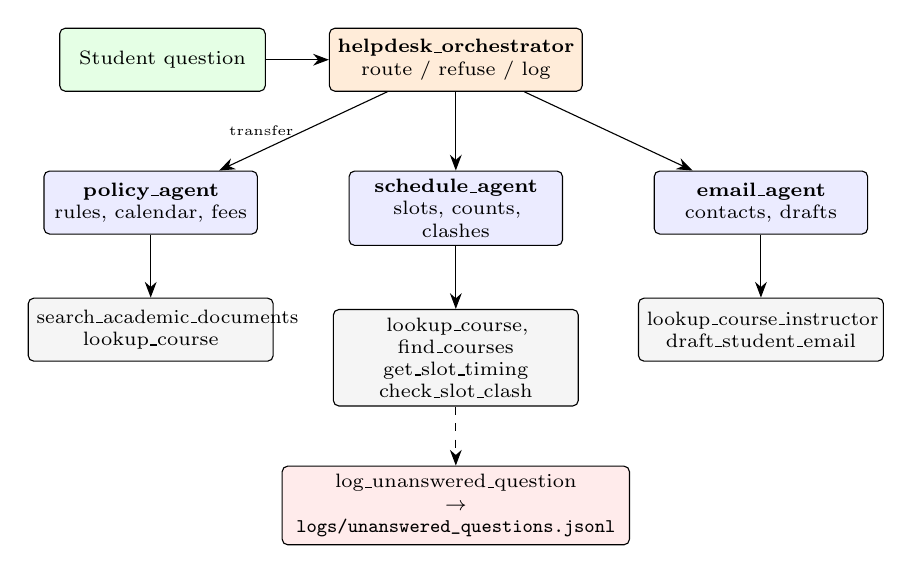
\begin{tikzpicture}[
  node distance=0.55cm and 0.5cm,
  box/.style={draw,rounded corners=2pt,align=center,minimum height=0.8cm,font=\scriptsize,inner sep=3pt},
  agent/.style={box,fill=blue!8,text width=2.5cm},
  tool/.style={box,fill=black!4,text width=2.9cm},
  >={Stealth[length=2mm]}
]
\node[box,fill=green!10,text width=2.4cm] (q) {Student question};
\node[box,fill=orange!15,text width=3.0cm,right=0.8cm of q] (o) {\textbf{helpdesk\_orchestrator}\\route / refuse / log};
\node[agent,below left=1.0cm and 0.9cm of o] (p) {\textbf{policy\_agent}\\rules, calendar, fees};
\node[agent,below=1.0cm of o] (s) {\textbf{schedule\_agent}\\slots, counts, clashes};
\node[agent,below right=1.0cm and 0.9cm of o] (e) {\textbf{email\_agent}\\contacts, drafts};
\node[tool,below=0.8cm of p] (tp) {search\_academic\_documents\\lookup\_course};
\node[tool,below=0.8cm of s] (ts) {lookup\_course, find\_courses\\get\_slot\_timing\\check\_slot\_clash};
\node[tool,below=0.8cm of e] (te) {lookup\_course\_instructor\\draft\_student\_email};
\node[box,fill=red!8,text width=4.2cm,below=0.75cm of ts] (log) {log\_unanswered\_question\\$\rightarrow$ \code{logs/unanswered_questions.jsonl}};
\draw[->] (q) -- (o);
\draw[->] (o) -- node[left,font=\tiny]{transfer} (p);
\draw[->] (o) -- (s);
\draw[->] (o) -- (e);
\draw[->] (p) -- (tp);
\draw[->] (s) -- (ts);
\draw[->] (e) -- (te);
\draw[->,dashed] (ts) -- (log);
\end{tikzpicture}
\caption{Multi-agent architecture. The orchestrator transfers in-scope questions to one specialist and handles out-of-scope questions itself; every refusal calls the logging tool. Each specialist also has access to the logging tool (not drawn).}\label{fig:arch}
\end{figure}

\begin{table}[H]
\centering\small
\caption{Agents, responsibilities and tools.}\label{tab:agents}
\begin{tabularx}{\textwidth}{@{}l Y Y@{}}
\toprule
\textbf{Agent} & \textbf{Responsibility} & \textbf{Tools}\\
\midrule
Orchestrator & Route to exactly one specialist; refuse out-of-scope questions without delegating & \code{log_unanswered_question}, transfer\\
Policy agent & Rules, regulations, calendar, fees, curriculum; at most two searches per question & \code{search_academic_documents}, \code{lookup_course}, \code{log_unanswered_question}\\
Schedule agent & Slots, timings, rooms, counts, clashes; reports tool counts verbatim & \code{lookup_course}, \code{find_courses}, \code{get_slot_timing}, \code{check_slot_clash}, \code{search_academic_documents}, \code{log_unanswered_question}\\
Email agent & Instructor lookup and a draft for review; never sends & \code{lookup_course_instructor}, \code{draft_student_email}, \code{log_unanswered_question}\\
\bottomrule
\end{tabularx}
\end{table}

\begin{figure}[H]
\centering
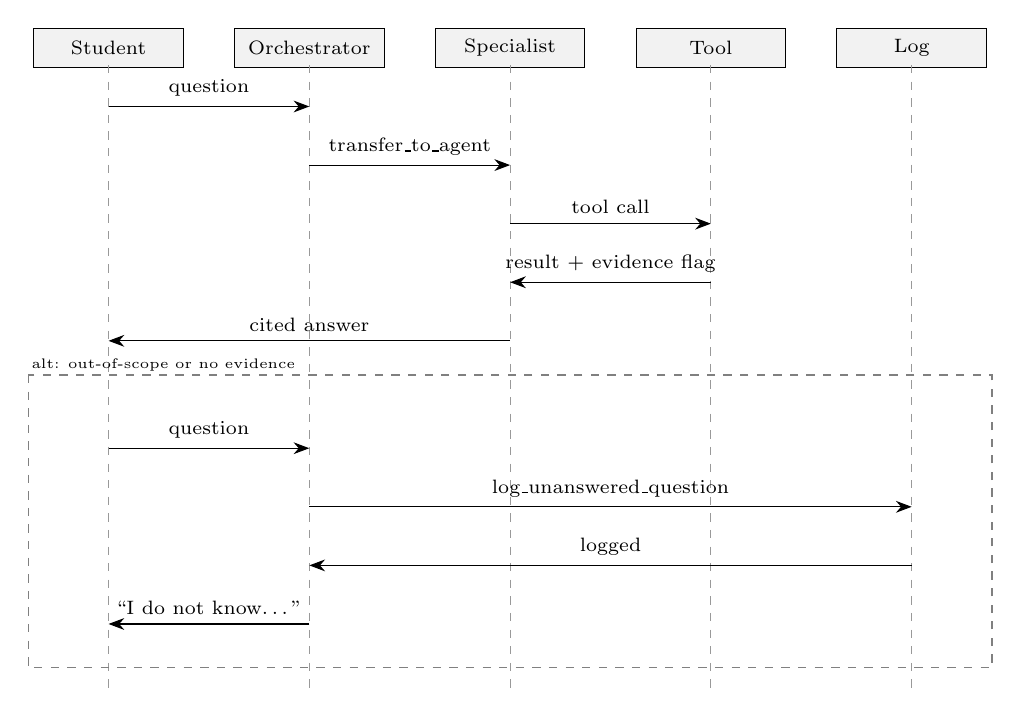
\begin{tikzpicture}[x=2.55cm,y=-0.62cm,font=\scriptsize,>={Stealth[length=2mm]}]
  \foreach \x/\n in {0/Student,1/Orchestrator,2/Specialist,3/Tool,4/Log}{
    \node[draw,fill=black!5,minimum width=1.9cm,minimum height=0.5cm] (n\x) at (\x,0) {\n};
    \draw[dashed,black!40] (\x,0.35) -- (\x,13.2);
  }
  \draw[->] (0,1.2) -- node[above]{question} (1,1.2);
  \draw[->] (1,2.4) -- node[above]{transfer\_to\_agent} (2,2.4);
  \draw[->] (2,3.6) -- node[above]{tool call} (3,3.6);
  \draw[<-] (2,4.8) -- node[above]{result + evidence flag} (3,4.8);
  \draw[->] (2,6.0) -- node[above]{cited answer} (0,6.0);
  \draw[dashed,black!50] (-0.4,6.7) rectangle (4.4,12.7);
  \node[font=\tiny,anchor=south west,inner sep=1pt] at (-0.4,6.7) {alt: out-of-scope or no evidence};
  \draw[->] (0,8.2) -- node[above]{question} (1,8.2);
  \draw[->] (1,9.4) -- node[above]{log\_unanswered\_question} (4,9.4);
  \draw[<-] (1,10.6) -- node[above]{logged} (4,10.6);
  \draw[->] (1,11.8) -- node[above]{``I do not know\ldots''} (0,11.8);
\end{tikzpicture}
\caption{Sequence of one turn. Upper block: an in-scope question is delegated, the specialist calls a tool and answers with citations. Lower block: an out-of-scope question (or one where \code{sufficient_evidence} is false) is logged and refused.}\label{fig:seq}
\end{figure}

% =====================================================================
\section{Core Pipeline: Hybrid, Authority-Aware Retrieval}\label{sec:pipeline}
% =====================================================================
\textbf{Index.} The 390 chunks are embedded with the all-MiniLM-L6-v2 model (384 dimensions). Chunk length is 301 to 17,767 characters (median 4,094; mean 4,031). The chunking parameters used when the shared index was built are not recorded in the repository; the statistics above were measured from the stored chunks. The stored vectors were loaded as they are; the query embedder reproduces them with mean cosine similarity 1.0000 on a 12-chunk sample, confirming that queries and documents share one embedding space.

\textbf{Retrieval.} For a question $q$ the search tool (Figure~\ref{fig:pipe}) proceeds as follows.
\begin{enumerate}
  \item Embed $q$ and take the 60 nearest chunks by cosine distance $d$ (\code{CANDIDATE_K}=60).
  \item Add up to 12 further chunks whose keyword coverage is at least 0.6. Coverage is the IDF-weighted share of the question's distinctive words found in the chunk, with $\mathrm{idf}(w)=\ln\frac{N+1}{\mathrm{df}(w)+0.5}$ over the 390 chunks and a high weight for words absent from the corpus. This recovers scanned or noisy pages that embed poorly.
  \item Score each candidate: $s = (1-d) + b_{\mathrm{id}} + 0.2\,c + 0.3\,[c\ge0.95 \wedge n_w\ge2] + a$, where $b_{\mathrm{id}}\le0.30$ rewards identifier overlap (course codes), $c$ is coverage, $n_w$ the number of distinctive query words, and $a$ is an authority adjustment: $+0.12$ for a document that supersedes others on a topic the question mentions and $-0.06$ for a document it supersedes, taken from \code{doc_authority.csv}.
  \item Return the top 3 chunks (\code{TOP_K}=3). Each is trimmed to the most relevant window by the IDF weight of the query words it contains; the three share a budget of $3\times1000$ characters, with the top hit allowed up to 1,800.
  \item Mark the evidence \emph{sufficient} if the best distance is at most 0.50 (\code{MAX_RELEVANT_DISTANCE}), or if some chunk has coverage $\ge0.95$ and the question has at least two distinctive words.
\end{enumerate}

\begin{figure}[H]
\centering
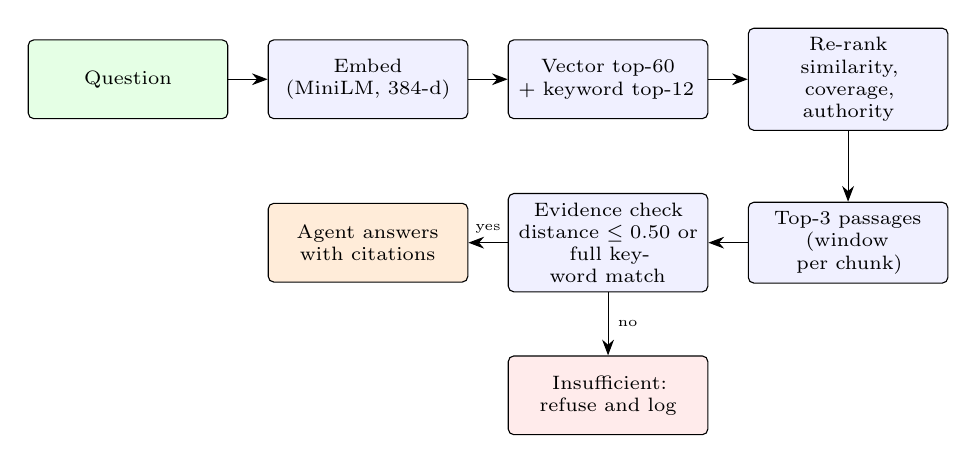
\begin{tikzpicture}[node distance=0.45cm and 0.5cm,
  box/.style={draw,rounded corners=2pt,align=center,font=\scriptsize,text width=2.3cm,minimum height=1.0cm,fill=blue!6},
  >={Stealth[length=2mm]}]
\node[box,fill=green!10] (a) {Question};
\node[box,right=of a] (b) {Embed\\(MiniLM, 384-d)};
\node[box,right=of b] (c) {Vector top-60\\+ keyword top-12};
\node[box,right=of c] (d) {Re-rank\\similarity, coverage,\\authority};
\node[box,below=0.9cm of d] (e) {Top-3 passages\\(window per chunk)};
\node[box,left=of e] (f) {Evidence check\\distance $\le0.50$ or\\full keyword match};
\node[box,left=of f,fill=orange!15] (g) {Agent answers\\with citations};
\node[box,below=0.8cm of f,fill=red!8] (h) {Insufficient:\\refuse and log};
\draw[->] (a)--(b); \draw[->] (b)--(c); \draw[->] (c)--(d); \draw[->] (d)--(e);
\draw[->] (e)--(f); \draw[->] (f)--node[above,font=\tiny]{yes}(g); \draw[->] (f)--node[right,font=\tiny]{no}(h);
\end{tikzpicture}
\caption{Retrieval pipeline from question to cited answer or logged refusal.}\label{fig:pipe}
\end{figure}

\textbf{Component-level check.} On the 11 document-backed questions the expected document appears at rank 1 for 10 of 11 questions (hit@1 = hit@3 = hit@5 = 10/11) and within the top 10 for all 11 (hit@10 = 11/11), giving mean reciprocal rank (MRR) 0.918 (Table~\ref{tab:rank}). The one question outside the top 3 is Q11, which has no decisive document (Section~\ref{sec:limits}). Retrieval is therefore not the main source of later failures; what the model is shown from the retrieved chunks, and its own use of it, is.

\begin{table}[H]
\centering\small
\caption{Retrieval ranking on the 11 document-backed questions (question text used as the query).}\label{tab:rank}
\begin{tabular}{@{}lcccc@{}}
\toprule
\textbf{hit@1} & \textbf{hit@3} & \textbf{hit@5} & \textbf{hit@10} & \textbf{MRR}\\
\midrule
10/11 (90.9\%) & 10/11 & 10/11 & 11/11 (100\%) & 0.918\\
\bottomrule
\end{tabular}
\end{table}

% =====================================================================
\section{Implementation}\label{sec:impl}
% =====================================================================
\textbf{Setup and hardware.} The system was developed on Windows~11 with 16~GB RAM and no GPU use: chat inference is remote. Software: Python 3.12, Google ADK 2.13.0, LiteLLM 1.106.6, ONNX Runtime 1.20.1 (newer versions failed to initialise on the development machine), NumPy, FastAPI and React for the demo. The chat model is configured by one string (\code{HELPDESK_MODEL}); the models used are \code{groq/qwen/qwen3.8-27b} (primary) and \code{groq/openai/gpt-oss-20b}. Embeddings run locally, because the hosted provider offers no embeddings endpoint. The vector store is an exact cosine search over the 390 vectors (a NumPy backend selectable with \code{VECTOR_BACKEND=numpy}), used because ChromaDB's native index crashed on the development machine; for 390 vectors the choice does not change results.

\textbf{Grounding and citation policy.} Every fact must come from a tool result. Answers end with a \code{Sources:} line giving the document identifier, title and page range (for documents) or the CSV file (for tool data). The prompts forbid inventing identifiers, clauses, course codes, emails, rooms, dates or counts, and say that when documents of different dates disagree the later circular is preferred and both are cited.

\textbf{Deterministic versus model-enforced behaviour.}
\begin{table}[H]
\centering\small
\caption{What is enforced by code and what is left to the model.}\label{tab:enforce}
\begin{tabularx}{\textwidth}{@{}lYY@{}}
\toprule
\textbf{Behaviour} & \textbf{Enforced by code} & \textbf{Left to the model}\\
\midrule
Counts, slots, rooms, credits & CSV tools return \code{match_count}/\code{course_count}; current semester only & reporting the tool's number verbatim\\
Instructor email & looked up by course code; unknown code returns not found & not inventing an address\\
Email draft & template rendered by code; quotes no clause or form; status \code{draft_not_sent} & choosing the request type and arguments\\
Retrieval verdict & \code{sufficient_evidence} flag & obeying it\\
Out-of-scope refusal & orchestrator holds no answering tools & recognising the topic as out of scope\\
Refusal logging & \code{log_unanswered_question} appends to the log & calling it\\
\bottomrule
\end{tabularx}
\end{table}

\textbf{Repository layout.}
\begin{table}[H]
\centering\small
\caption{Repository layout.}\label{tab:layout}
\begin{tabularx}{\textwidth}{@{}l Y@{}}
\toprule
\textbf{Path} & \textbf{Contents}\\
\midrule
\code{academic_helpdesk/} & agent graph and single-agent baseline (\code{agent.py}), prompts, programmatic driver (\code{runner.py}), terminal client, rate-limit-aware model client, configuration\\
\code{academic_helpdesk/rag/} & retrieval and re-ranking (\code{store.py}), loader for the prebuilt index, exact-search store, extraction and chunking utilities\\
\code{academic_helpdesk/tools/} & search, schedule, contact, email and escalation tools; CSV loading\\
\code{data1/} & prebuilt index (\code{chroma/}), structured CSVs (\code{structured/}), source manifest\\
\code{eval/} & question set, scoring harness, deterministic checks, evidence evaluation, report-asset generator\\
\code{web/} & FastAPI service (\code{backend/service.py}) and React interface (\code{frontend/})\\
\code{report/} & this report\\
\bottomrule
\end{tabularx}
\end{table}

\textbf{Web demo.} A browser interface runs the same code path as the terminal client and the evaluation harness. A FastAPI service exposes \code{/api/chat/stream}, which streams each step of a turn as server-sent events (agent hand-offs, tool calls, retrieved documents and rate-limit waits), together with \code{/api/search} (retrieval only), \code{/api/status}, \code{/api/reset}, \code{/api/unanswered} and \code{/api/email-drafts}. The React interface has four views: a chat with a live step timeline, source chips, a flow diagram and an email-draft card; a \emph{Scenarios} tab that runs the assignment's seven example questions and checks the route, the tools called, the citation, the draft status and the logged refusal; an \emph{Evidence} tab showing the ranked chunks, their distances and the sufficiency verdict; and a \emph{Logs} tab reading the unanswered-question and email-draft logs. The interface was exercised through its streaming endpoint (the email and course-count questions) and its production build; it was not covered by automated browser tests.

\textbf{Rate limits.} The hosted free tier caps the Qwen model at about 7,000 input tokens per minute for the whole account. A client wrapper reads the wait time from each rate-limit response (seconds, milliseconds or minutes) and retries, so a turn is delayed but not lost.

\textbf{Security notes.} Drafts are never sent and no mail credentials exist. The system has no access to any student's record. The hosted-model API key was committed to the repository in an early commit; it is untracked and git-ignored now but remains in history and must be rotated by the repository owner; this report does not claim that has been done.

% =====================================================================
\section{Evaluation Methodology}\label{sec:evalmethod}
% =====================================================================
\textbf{Question set.} 30 questions (Appendix~A): 11 rules and calendar (Q01--Q11), 9 timetable and offerings (Q12--Q20), 5 email (Q21--Q25) and 5 out of scope (Q26--Q30). Reference answers for document questions were read from the source documents; schedule and email answers were derived from the CSVs by code. Q11 (Open Elective credits) is a deliberate limit case: the curricula list Programme and Open Electives together and state no separate total, so an honest ``not specified'' or a refusal scores correct and an invented number does not.

\textbf{Two evaluations.}
\begin{enumerate}
  \item \emph{Evidence evaluation} (no model). For each question the retrieval or tool step is run exactly as an agent would call it, and three checks are made: the right document or record is found; the required facts are present in the evidence the model would see; and the sufficiency verdict is right (answerable $\to$ sufficient, out of scope $\to$ insufficient). This bounds what any model can achieve; it is not a model score.
  \item \emph{Model evaluation.} The full multi-agent system answers each question in a fresh session. Configurations planned: Qwen3.8-27B multi-agent, 3 repetitions; gpt-oss-20B multi-agent, 2 repetitions. Planned graded outputs: $3\times30+2\times30=150$. At the time of writing no graded output had been completed (Section~\ref{sec:results}). The single-agent baseline exists but was not evaluated.
\end{enumerate}

\textbf{Ablations performed.} (i) Four retrieval variants, measured by expected-document rank and false refusals (Table~\ref{tab:retr}). (ii) Prompt and tool-definition trimming, measured by per-call request size and turn time (Table~\ref{tab:tokens}). No component ablation was run on the model.

\textbf{Metrics and scoring.} All scoring is by deterministic rules; \textbf{no language-model judge is used}, so there is no judge subjectivity, but the rules are strict (Section~\ref{sec:limits}). Text is normalised (Unicode NFKC, dash and quote folding) before comparison.
\begin{itemize}
  \item \emph{Accuracy:} every entry of \code{must_contain} is present (a list entry means any one option) and no \code{must_not_contain} entry is; for refusal questions, the answer is a refusal.
  \item \emph{Groundedness:} an accurate answer that cites at least one expected source identifier and cites no identifier absent from the corpus (invented slugs in the \code{Sources:} section are detected).
  \item \emph{Correct refusal / false refusal:} share of the 5 out-of-scope questions refused / share of answerable questions refused.
  \item \emph{Routing:} share of questions delegated to the expected specialist (none for out-of-scope).
  \item \emph{Consistency:} questions whose verdict differs between repetitions.
\end{itemize}

% =====================================================================
\section{Results}\label{sec:results}
% =====================================================================
\subsection{Evidence evaluation (all 30 questions, no model)}
\begin{table}[H]
\centering\small
\caption{Evidence evaluation by category. n/a: the check does not apply.}\label{tab:evidence}
\begin{tabular}{@{}lrrr@{}}
\toprule
\textbf{Category (questions)} & \textbf{Document/record found} & \textbf{Facts in evidence} & \textbf{Verdict right}\\
\midrule
Rules and calendar (11) & 10/11 & 10/11 & 11/11\\
Timetable (9) & 9/9 & 9/9 & n/a\\
Email (5) & 5/5 & 5/5 & n/a\\
Out of scope (5) & n/a & n/a & 4/5\\
\midrule
\textbf{All applicable} & \textbf{24/25 (96\%)} & \textbf{24/25 (96\%)} & \textbf{15/16 (93.8\%)}\\
\bottomrule
\end{tabular}

\smallskip
\footnotesize Q11 is the limit case (no decisive document); Q27 passes the evidence check, so its refusal depends on the orchestrator's scope rule.
\end{table}

\begin{figure}[H]
\centering
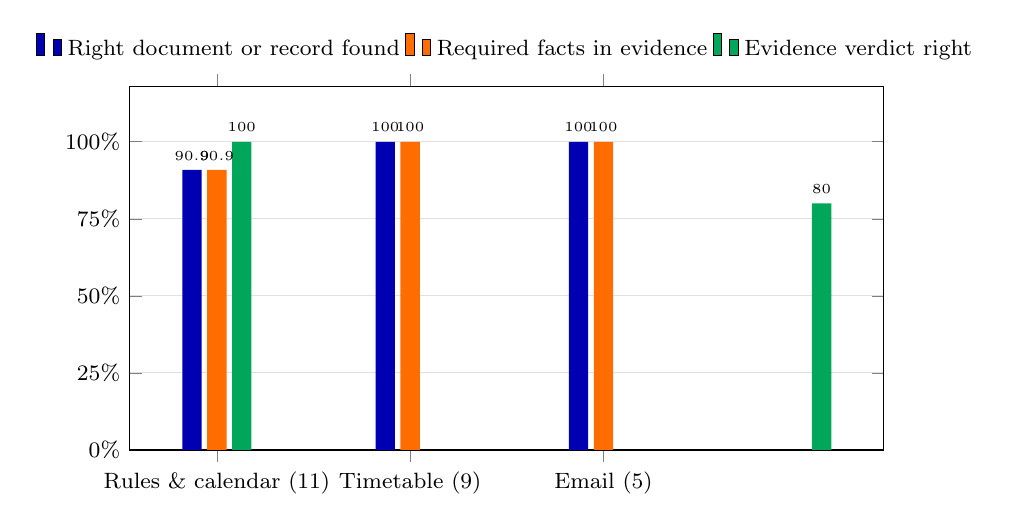
\begin{tikzpicture}
\begin{axis}[
  ybar,bar width=7pt,width=0.92\textwidth,height=6.2cm,
  symbolic x coords={Rules,Timetable,Email,Refuse},
  xtick=data,xticklabels={Rules \& calendar (11),Timetable (9),Email (5),Must refuse (5)},
  ymin=0,ymax=118,ytick={0,25,50,75,100},yticklabel={\pgfmathprintnumber{\tick}\%},
  ymajorgrids,grid style={black!12},tick label style={font=\footnotesize},
  legend style={at={(0.5,1.04)},anchor=south,legend columns=-1,font=\footnotesize,draw=none},
  nodes near coords,every node near coord/.append style={font=\tiny},
  nodes near coords align={vertical},enlarge x limits=0.15]
\addplot[fill=blue!70!black,draw=none] coordinates {(Rules,90.9) (Timetable,100) (Email,100)};
\addplot[fill=orange!85!red,draw=none] coordinates {(Rules,90.9) (Timetable,100) (Email,100)};
\addplot[fill=teal!70!green,draw=none] coordinates {(Rules,100) (Refuse,80)};
\legend{Right document or record found,Required facts in evidence,Evidence verdict right}
\end{axis}
\end{tikzpicture}
\caption{Evidence handed to the model, by question category (no model involved). Timetable and email evidence is complete because it comes from deterministic tools; the policy shortfall is the Q11 limit case.}\label{fig:evbar}
\end{figure}

\begin{figure}[H]
\centering
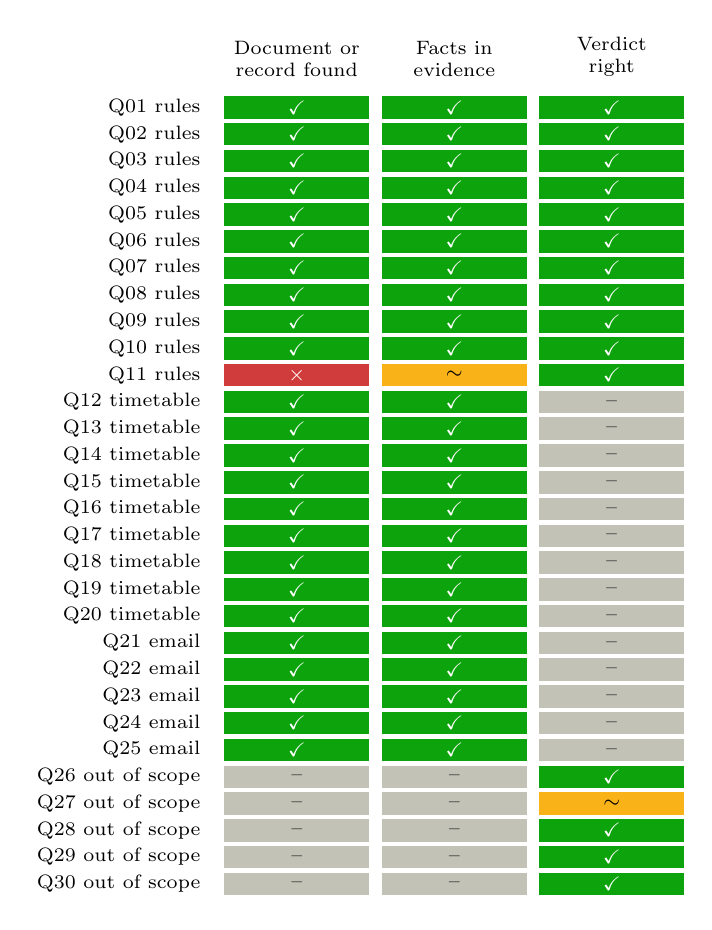
\begin{tikzpicture}[x=2.0cm,y=-0.34cm,font=\scriptsize]
  \node[align=center,anchor=south] at (0.5,-0.3) {Document or\\record found};
  \node[align=center,anchor=south] at (1.5,-0.3) {Facts in\\evidence};
  \node[align=center,anchor=south] at (2.5,-0.3) {Verdict\\right};
  \node[anchor=east] at (-0.05,0.5) {Q01\ rules};
  \fill[good] (0.04,0.08) rectangle (0.96,0.92);
  \node[text=white] at (0.5,0.5) {\checkmark};
  \fill[good] (1.04,0.08) rectangle (1.96,0.92);
  \node[text=white] at (1.5,0.5) {\checkmark};
  \fill[good] (2.04,0.08) rectangle (2.96,0.92);
  \node[text=white] at (2.5,0.5) {\checkmark};
  \node[anchor=east] at (-0.05,1.5) {Q02\ rules};
  \fill[good] (0.04,1.08) rectangle (0.96,1.92);
  \node[text=white] at (0.5,1.5) {\checkmark};
  \fill[good] (1.04,1.08) rectangle (1.96,1.92);
  \node[text=white] at (1.5,1.5) {\checkmark};
  \fill[good] (2.04,1.08) rectangle (2.96,1.92);
  \node[text=white] at (2.5,1.5) {\checkmark};
  \node[anchor=east] at (-0.05,2.5) {Q03\ rules};
  \fill[good] (0.04,2.08) rectangle (0.96,2.92);
  \node[text=white] at (0.5,2.5) {\checkmark};
  \fill[good] (1.04,2.08) rectangle (1.96,2.92);
  \node[text=white] at (1.5,2.5) {\checkmark};
  \fill[good] (2.04,2.08) rectangle (2.96,2.92);
  \node[text=white] at (2.5,2.5) {\checkmark};
  \node[anchor=east] at (-0.05,3.5) {Q04\ rules};
  \fill[good] (0.04,3.08) rectangle (0.96,3.92);
  \node[text=white] at (0.5,3.5) {\checkmark};
  \fill[good] (1.04,3.08) rectangle (1.96,3.92);
  \node[text=white] at (1.5,3.5) {\checkmark};
  \fill[good] (2.04,3.08) rectangle (2.96,3.92);
  \node[text=white] at (2.5,3.5) {\checkmark};
  \node[anchor=east] at (-0.05,4.5) {Q05\ rules};
  \fill[good] (0.04,4.08) rectangle (0.96,4.92);
  \node[text=white] at (0.5,4.5) {\checkmark};
  \fill[good] (1.04,4.08) rectangle (1.96,4.92);
  \node[text=white] at (1.5,4.5) {\checkmark};
  \fill[good] (2.04,4.08) rectangle (2.96,4.92);
  \node[text=white] at (2.5,4.5) {\checkmark};
  \node[anchor=east] at (-0.05,5.5) {Q06\ rules};
  \fill[good] (0.04,5.08) rectangle (0.96,5.92);
  \node[text=white] at (0.5,5.5) {\checkmark};
  \fill[good] (1.04,5.08) rectangle (1.96,5.92);
  \node[text=white] at (1.5,5.5) {\checkmark};
  \fill[good] (2.04,5.08) rectangle (2.96,5.92);
  \node[text=white] at (2.5,5.5) {\checkmark};
  \node[anchor=east] at (-0.05,6.5) {Q07\ rules};
  \fill[good] (0.04,6.08) rectangle (0.96,6.92);
  \node[text=white] at (0.5,6.5) {\checkmark};
  \fill[good] (1.04,6.08) rectangle (1.96,6.92);
  \node[text=white] at (1.5,6.5) {\checkmark};
  \fill[good] (2.04,6.08) rectangle (2.96,6.92);
  \node[text=white] at (2.5,6.5) {\checkmark};
  \node[anchor=east] at (-0.05,7.5) {Q08\ rules};
  \fill[good] (0.04,7.08) rectangle (0.96,7.92);
  \node[text=white] at (0.5,7.5) {\checkmark};
  \fill[good] (1.04,7.08) rectangle (1.96,7.92);
  \node[text=white] at (1.5,7.5) {\checkmark};
  \fill[good] (2.04,7.08) rectangle (2.96,7.92);
  \node[text=white] at (2.5,7.5) {\checkmark};
  \node[anchor=east] at (-0.05,8.5) {Q09\ rules};
  \fill[good] (0.04,8.08) rectangle (0.96,8.92);
  \node[text=white] at (0.5,8.5) {\checkmark};
  \fill[good] (1.04,8.08) rectangle (1.96,8.92);
  \node[text=white] at (1.5,8.5) {\checkmark};
  \fill[good] (2.04,8.08) rectangle (2.96,8.92);
  \node[text=white] at (2.5,8.5) {\checkmark};
  \node[anchor=east] at (-0.05,9.5) {Q10\ rules};
  \fill[good] (0.04,9.08) rectangle (0.96,9.92);
  \node[text=white] at (0.5,9.5) {\checkmark};
  \fill[good] (1.04,9.08) rectangle (1.96,9.92);
  \node[text=white] at (1.5,9.5) {\checkmark};
  \fill[good] (2.04,9.08) rectangle (2.96,9.92);
  \node[text=white] at (2.5,9.5) {\checkmark};
  \node[anchor=east] at (-0.05,10.5) {Q11\ rules};
  \fill[crit] (0.04,10.08) rectangle (0.96,10.92);
  \node[text=white] at (0.5,10.5) {$\times$};
  \fill[warn] (1.04,10.08) rectangle (1.96,10.92);
  \node[text=black] at (1.5,10.5) {$\sim$};
  \fill[good] (2.04,10.08) rectangle (2.96,10.92);
  \node[text=white] at (2.5,10.5) {\checkmark};
  \node[anchor=east] at (-0.05,11.5) {Q12\ timetable};
  \fill[good] (0.04,11.08) rectangle (0.96,11.92);
  \node[text=white] at (0.5,11.5) {\checkmark};
  \fill[good] (1.04,11.08) rectangle (1.96,11.92);
  \node[text=white] at (1.5,11.5) {\checkmark};
  \fill[neutral] (2.04,11.08) rectangle (2.96,11.92);
  \node[text=black] at (2.5,11.5) {--};
  \node[anchor=east] at (-0.05,12.5) {Q13\ timetable};
  \fill[good] (0.04,12.08) rectangle (0.96,12.92);
  \node[text=white] at (0.5,12.5) {\checkmark};
  \fill[good] (1.04,12.08) rectangle (1.96,12.92);
  \node[text=white] at (1.5,12.5) {\checkmark};
  \fill[neutral] (2.04,12.08) rectangle (2.96,12.92);
  \node[text=black] at (2.5,12.5) {--};
  \node[anchor=east] at (-0.05,13.5) {Q14\ timetable};
  \fill[good] (0.04,13.08) rectangle (0.96,13.92);
  \node[text=white] at (0.5,13.5) {\checkmark};
  \fill[good] (1.04,13.08) rectangle (1.96,13.92);
  \node[text=white] at (1.5,13.5) {\checkmark};
  \fill[neutral] (2.04,13.08) rectangle (2.96,13.92);
  \node[text=black] at (2.5,13.5) {--};
  \node[anchor=east] at (-0.05,14.5) {Q15\ timetable};
  \fill[good] (0.04,14.08) rectangle (0.96,14.92);
  \node[text=white] at (0.5,14.5) {\checkmark};
  \fill[good] (1.04,14.08) rectangle (1.96,14.92);
  \node[text=white] at (1.5,14.5) {\checkmark};
  \fill[neutral] (2.04,14.08) rectangle (2.96,14.92);
  \node[text=black] at (2.5,14.5) {--};
  \node[anchor=east] at (-0.05,15.5) {Q16\ timetable};
  \fill[good] (0.04,15.08) rectangle (0.96,15.92);
  \node[text=white] at (0.5,15.5) {\checkmark};
  \fill[good] (1.04,15.08) rectangle (1.96,15.92);
  \node[text=white] at (1.5,15.5) {\checkmark};
  \fill[neutral] (2.04,15.08) rectangle (2.96,15.92);
  \node[text=black] at (2.5,15.5) {--};
  \node[anchor=east] at (-0.05,16.5) {Q17\ timetable};
  \fill[good] (0.04,16.08) rectangle (0.96,16.92);
  \node[text=white] at (0.5,16.5) {\checkmark};
  \fill[good] (1.04,16.08) rectangle (1.96,16.92);
  \node[text=white] at (1.5,16.5) {\checkmark};
  \fill[neutral] (2.04,16.08) rectangle (2.96,16.92);
  \node[text=black] at (2.5,16.5) {--};
  \node[anchor=east] at (-0.05,17.5) {Q18\ timetable};
  \fill[good] (0.04,17.08) rectangle (0.96,17.92);
  \node[text=white] at (0.5,17.5) {\checkmark};
  \fill[good] (1.04,17.08) rectangle (1.96,17.92);
  \node[text=white] at (1.5,17.5) {\checkmark};
  \fill[neutral] (2.04,17.08) rectangle (2.96,17.92);
  \node[text=black] at (2.5,17.5) {--};
  \node[anchor=east] at (-0.05,18.5) {Q19\ timetable};
  \fill[good] (0.04,18.08) rectangle (0.96,18.92);
  \node[text=white] at (0.5,18.5) {\checkmark};
  \fill[good] (1.04,18.08) rectangle (1.96,18.92);
  \node[text=white] at (1.5,18.5) {\checkmark};
  \fill[neutral] (2.04,18.08) rectangle (2.96,18.92);
  \node[text=black] at (2.5,18.5) {--};
  \node[anchor=east] at (-0.05,19.5) {Q20\ timetable};
  \fill[good] (0.04,19.08) rectangle (0.96,19.92);
  \node[text=white] at (0.5,19.5) {\checkmark};
  \fill[good] (1.04,19.08) rectangle (1.96,19.92);
  \node[text=white] at (1.5,19.5) {\checkmark};
  \fill[neutral] (2.04,19.08) rectangle (2.96,19.92);
  \node[text=black] at (2.5,19.5) {--};
  \node[anchor=east] at (-0.05,20.5) {Q21\ email};
  \fill[good] (0.04,20.08) rectangle (0.96,20.92);
  \node[text=white] at (0.5,20.5) {\checkmark};
  \fill[good] (1.04,20.08) rectangle (1.96,20.92);
  \node[text=white] at (1.5,20.5) {\checkmark};
  \fill[neutral] (2.04,20.08) rectangle (2.96,20.92);
  \node[text=black] at (2.5,20.5) {--};
  \node[anchor=east] at (-0.05,21.5) {Q22\ email};
  \fill[good] (0.04,21.08) rectangle (0.96,21.92);
  \node[text=white] at (0.5,21.5) {\checkmark};
  \fill[good] (1.04,21.08) rectangle (1.96,21.92);
  \node[text=white] at (1.5,21.5) {\checkmark};
  \fill[neutral] (2.04,21.08) rectangle (2.96,21.92);
  \node[text=black] at (2.5,21.5) {--};
  \node[anchor=east] at (-0.05,22.5) {Q23\ email};
  \fill[good] (0.04,22.08) rectangle (0.96,22.92);
  \node[text=white] at (0.5,22.5) {\checkmark};
  \fill[good] (1.04,22.08) rectangle (1.96,22.92);
  \node[text=white] at (1.5,22.5) {\checkmark};
  \fill[neutral] (2.04,22.08) rectangle (2.96,22.92);
  \node[text=black] at (2.5,22.5) {--};
  \node[anchor=east] at (-0.05,23.5) {Q24\ email};
  \fill[good] (0.04,23.08) rectangle (0.96,23.92);
  \node[text=white] at (0.5,23.5) {\checkmark};
  \fill[good] (1.04,23.08) rectangle (1.96,23.92);
  \node[text=white] at (1.5,23.5) {\checkmark};
  \fill[neutral] (2.04,23.08) rectangle (2.96,23.92);
  \node[text=black] at (2.5,23.5) {--};
  \node[anchor=east] at (-0.05,24.5) {Q25\ email};
  \fill[good] (0.04,24.08) rectangle (0.96,24.92);
  \node[text=white] at (0.5,24.5) {\checkmark};
  \fill[good] (1.04,24.08) rectangle (1.96,24.92);
  \node[text=white] at (1.5,24.5) {\checkmark};
  \fill[neutral] (2.04,24.08) rectangle (2.96,24.92);
  \node[text=black] at (2.5,24.5) {--};
  \node[anchor=east] at (-0.05,25.5) {Q26\ out of scope};
  \fill[neutral] (0.04,25.08) rectangle (0.96,25.92);
  \node[text=black] at (0.5,25.5) {--};
  \fill[neutral] (1.04,25.08) rectangle (1.96,25.92);
  \node[text=black] at (1.5,25.5) {--};
  \fill[good] (2.04,25.08) rectangle (2.96,25.92);
  \node[text=white] at (2.5,25.5) {\checkmark};
  \node[anchor=east] at (-0.05,26.5) {Q27\ out of scope};
  \fill[neutral] (0.04,26.08) rectangle (0.96,26.92);
  \node[text=black] at (0.5,26.5) {--};
  \fill[neutral] (1.04,26.08) rectangle (1.96,26.92);
  \node[text=black] at (1.5,26.5) {--};
  \fill[warn] (2.04,26.08) rectangle (2.96,26.92);
  \node[text=black] at (2.5,26.5) {$\sim$};
  \node[anchor=east] at (-0.05,27.5) {Q28\ out of scope};
  \fill[neutral] (0.04,27.08) rectangle (0.96,27.92);
  \node[text=black] at (0.5,27.5) {--};
  \fill[neutral] (1.04,27.08) rectangle (1.96,27.92);
  \node[text=black] at (1.5,27.5) {--};
  \fill[good] (2.04,27.08) rectangle (2.96,27.92);
  \node[text=white] at (2.5,27.5) {\checkmark};
  \node[anchor=east] at (-0.05,28.5) {Q29\ out of scope};
  \fill[neutral] (0.04,28.08) rectangle (0.96,28.92);
  \node[text=black] at (0.5,28.5) {--};
  \fill[neutral] (1.04,28.08) rectangle (1.96,28.92);
  \node[text=black] at (1.5,28.5) {--};
  \fill[good] (2.04,28.08) rectangle (2.96,28.92);
  \node[text=white] at (2.5,28.5) {\checkmark};
  \node[anchor=east] at (-0.05,29.5) {Q30\ out of scope};
  \fill[neutral] (0.04,29.08) rectangle (0.96,29.92);
  \node[text=black] at (0.5,29.5) {--};
  \fill[neutral] (1.04,29.08) rectangle (1.96,29.92);
  \node[text=black] at (1.5,29.5) {--};
  \fill[good] (2.04,29.08) rectangle (2.96,29.92);
  \node[text=white] at (2.5,29.5) {\checkmark};
\end{tikzpicture}
\caption{Per-question evidence check (green check: yes; amber tilde: depends on the model or is a limit case; red cross: no; grey dash: not applicable). Only Q11 and Q27 are not fully green where a check applies.}\label{fig:evgrid}
\end{figure}

\subsection{Model-answer evaluation: status}
The model-answer evaluation specified in Section~\ref{sec:evalmethod} was started: Qwen3.8-27B multi-agent with 3 repetitions and gpt-oss-20B multi-agent with 2 repetitions, 150 graded outputs in all. When this report was written neither run had completed a single question. The cause is the hosted free tier: one question needs three to five model calls of 1,400 to 4,600 tokens each against a limit of about 8,000 tokens per minute, and the runs were repeatedly held back by rate-limit waits of 76 to 90 seconds. Consequently \textbf{no measured accuracy, groundedness, refusal-rate, routing or consistency figure for model answers is available.} Section~\ref{sec:estimates} gives explicitly hypothetical single-point estimates, which must not be interpreted as actual scores. The strongest statements the measurements support are the evidence evaluation above, the deterministic checks of Section~\ref{sec:results} and the four observed answers below.

\begin{table}[H]
\centering\small
\caption{Status of the model-answer evaluation at the time of writing.}\label{tab:status}
\begin{tabular}{@{}lccc@{}}
\toprule
\textbf{Configuration} & \textbf{Repetitions planned} & \textbf{Graded outputs planned} & \textbf{Completed}\\
\midrule
Qwen3.8-27B, multi-agent & 3 & 90 & 0\\
gpt-oss-20B, multi-agent & 2 & 60 & 0\\
Single-agent baseline & -- & -- & not run\\
\bottomrule
\end{tabular}
\end{table}

\subsection{Single-point model estimates (not measured)}\label{sec:estimates}
\textbf{All model-specific scores in this subsection are estimates, not measurements.} Because full model evaluation did not complete, illustrative integer counts of correct answers were assumed for each category. The percentages are calculated as $100k/n$ from those hypothetical counts, and overall accuracy uses the total correct answers out of 30. The point estimates are neither observed experimental results nor statistically calibrated predictions. One answer changes a category score by 9.1 points (rules), 11.1 points (timetable), or 20 points (email and refusal).

\begin{table}[H]
\centering\small
\caption{Basis of point estimates. Only the first row is a systematic measurement.}\label{tab:basis}
\begin{tabularx}{\textwidth}{@{}l Y l@{}}
\toprule
\textbf{Input} & \textbf{How it is used} & \textbf{Status}\\
\midrule
Evidence ceiling (Table~\ref{tab:evidence}) & No model can exceed the evidence it is given: rules 10 of 11 with facts present plus Q11 answerable by an honest ``not specified'', timetable 9 of 9, email 5 of 5, refusal 4 of 5 by evidence with Q27 left to the prompt & measured\\
Model reliability & Hypothetical integer correct-answer counts favour tool-based categories; an assumed model ordering is used for illustration but has not been experimentally established & assumption\\
Early observations & Qwen3.8-27B answered the 4 sampled questions correctly (Table~\ref{tab:observed}). A stopped partial run of \code{gpt-oss-20b} on Q01--Q10, made before the passage-window fix and whose log was not kept, gave 7 accurate, 6 grounded and 10 correctly routed & observed, not scored\\
Groundedness & Assumed correctly answered and cited counts of 22, 23 and 19 out of 30 for Qwen, 120B and 20B; all are below their corresponding accuracy counts & assumption\\
Run-to-run change & Assumed counts of changing verdicts across repetitions: 3, 2 and 5 respectively; no repetitions have been graded & assumption\\
\bottomrule
\end{tabularx}
\end{table}

\begin{table}[H]
\centering\small
\caption{\textbf{Estimated, not measured} accuracy by model and category. Each cell gives assumed correct answers and the corresponding percentage; overall uses all 30 questions.}\label{tab:matrix}
\scriptsize
\begin{tabular}{@{}lccccc@{}}
\toprule
\textbf{Model} & \textbf{Rules (11)} & \textbf{Timetable (9)} & \textbf{Email (5)} & \textbf{Refuse (5)} & \textbf{Overall (30)}\\
\midrule
Qwen3.8-27B & \cellcolor{orange!30}8/11 (72.7\%) & \cellcolor{yellow!35}8/9 (88.9\%) & \cellcolor{green!25}5/5 (100\%) & \cellcolor{yellow!35}4/5 (80\%) & \cellcolor{yellow!35}25/30 (83.3\%)\\
gpt-oss-120B & \cellcolor{yellow!35}9/11 (81.8\%) & \cellcolor{yellow!35}8/9 (88.9\%) & \cellcolor{green!25}5/5 (100\%) & \cellcolor{yellow!35}4/5 (80\%) & \cellcolor{yellow!35}26/30 (86.7\%)\\
gpt-oss-20B & \cellcolor{red!18}7/11 (63.6\%) & \cellcolor{orange!30}7/9 (77.8\%) & \cellcolor{yellow!35}4/5 (80\%) & \cellcolor{yellow!35}4/5 (80\%) & \cellcolor{orange!30}22/30 (73.3\%)\\
\bottomrule
\end{tabular}
\end{table}

\begin{figure}[H]
\centering
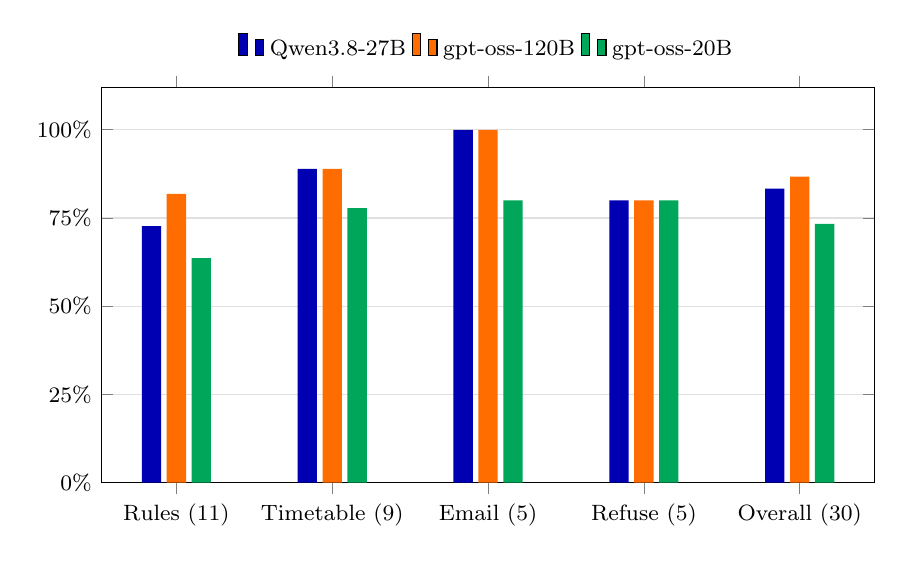
\begin{tikzpicture}
\begin{axis}[
  ybar,bar width=7pt,width=0.94\textwidth,height=6.6cm,
  symbolic x coords={Rules,Timetable,Email,Refuse,Overall},xtick=data,
  xticklabels={Rules (11),Timetable (9),Email (5),Refuse (5),Overall (30)},
  ymin=0,ymax=112,ytick={0,25,50,75,100},yticklabel={\pgfmathprintnumber{\tick}\%},
  ymajorgrids,grid style={black!12},tick label style={font=\footnotesize},
  legend style={at={(0.5,1.04)},anchor=south,legend columns=-1,font=\footnotesize,draw=none},
  enlarge x limits=0.12]
\addplot[fill=blue!70!black,draw=none] coordinates {(Rules,72.7) (Timetable,88.9) (Email,100) (Refuse,80) (Overall,83.3)};
\addplot[fill=orange!85!red,draw=none] coordinates {(Rules,81.8) (Timetable,88.9) (Email,100) (Refuse,80) (Overall,86.7)};
\addplot[fill=teal!70!green,draw=none] coordinates {(Rules,63.6) (Timetable,77.8) (Email,80) (Refuse,80) (Overall,73.3)};
\legend{Qwen3.8-27B,gpt-oss-120B,gpt-oss-20B}
\end{axis}
\end{tikzpicture}
\caption{\textbf{Estimated, not measured} accuracy by model and category. Bars show hypothetical single-point scores computed from the counts in Table~\ref{tab:matrix}; they do not establish a measured ranking.}\label{fig:estcat}
\end{figure}

\begin{table}[H]
\centering\small
\caption{\textbf{Estimated, not measured} overall accuracy, groundedness and run-to-run changes. All are illustrative assumptions.}\label{tab:estground}
\begin{tabular}{@{}lccc@{}}
\toprule
\textbf{Model} & \textbf{Accuracy (\%)} & \textbf{Groundedness (\%)} & \textbf{Questions changing between runs (of 30)}\\
\midrule
Qwen3.8-27B & 83.3 (25/30) & 73.3 (22/30) & 3\\
gpt-oss-120B & 86.7 (26/30) & 76.7 (23/30) & 2\\
gpt-oss-20B & 73.3 (22/30) & 63.3 (19/30) & 5\\
\bottomrule
\end{tabular}
\end{table}

\begin{figure}[H]
\centering
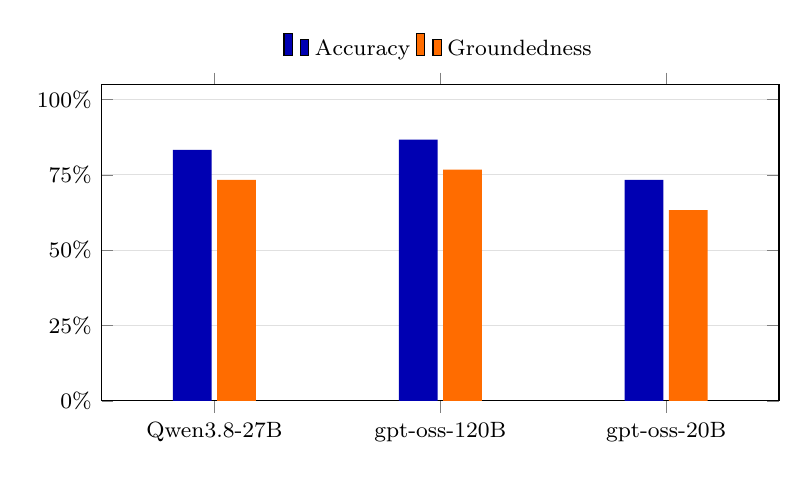
\begin{tikzpicture}
\begin{axis}[
  ybar,bar width=14pt,width=0.84\textwidth,height=5.6cm,
  symbolic x coords={Q,G120,G20},xtick=data,xticklabels={Qwen3.8-27B,gpt-oss-120B,gpt-oss-20B},
  ymin=0,ymax=105,ytick={0,25,50,75,100},yticklabel={\pgfmathprintnumber{\tick}\%},
  ymajorgrids,grid style={black!12},tick label style={font=\footnotesize},
  legend style={at={(0.5,1.04)},anchor=south,legend columns=-1,font=\footnotesize,draw=none},
  enlarge x limits=0.25]
\addplot[fill=blue!70!black,draw=none] coordinates {(Q,83.3) (G120,86.7) (G20,73.3)};
\addplot[fill=orange!85!red,draw=none] coordinates {(Q,73.3) (G120,76.7) (G20,63.3)};
\legend{Accuracy,Groundedness}
\end{axis}
\end{tikzpicture}
\caption{\textbf{Estimated, not measured} overall accuracy and groundedness. Bars are hypothetical counts divided by 30; groundedness additionally requires correct citations.}\label{fig:estground}
\end{figure}

\textbf{How to replace estimates with measurements.} Run the two evaluation commands of Section~\ref{sec:repro} (and the same for \code{groq/openai/gpt-oss-120b}), then \code{python eval/make_report_assets.py}; replace these illustrative counts and charts with measured outputs. Actual measurements always take precedence over the estimates.

\subsection{Observed model behaviour (not scored)}
Four answers were observed from the full system on \code{qwen/qwen3.8-27b}; they illustrate the intended behaviour and are not a sample.
\begin{table}[H]
\centering\small
\caption{Observed runs of the multi-agent system.}\label{tab:observed}
\begin{tabularx}{\textwidth}{@{}Y Y Y@{}}
\toprule
\textbf{Question} & \textbf{Route and tools} & \textbf{Outcome}\\
\midrule
Attendance requirement for the Major exam & orchestrator $\to$ policy agent; \code{search_academic_documents} & cited \code{amend_attendance_2024}; exam eligibility no longer tied to attendance; attendance should not fall below 75\%\\
Email to the CSL7570 instructor, 2 days' leave & orchestrator $\to$ email agent; \code{lookup_course_instructor}, \code{draft_student_email} & draft to \code{sranjan@iitj.ac.in}, placeholders for student details, marked not sent\\
400-level Humanities electives & orchestrator $\to$ schedule agent; \code{find_courses} & 7, with all seven courses listed, citing \code{courses.csv}\\
Dining options & orchestrator only & ``I do not know\ldots'', not delegated, logged as \code{out_of_scope}\\
\bottomrule
\end{tabularx}
\end{table}
One failure was also observed: after the prompts were shortened, the policy agent hedged on the attendance question and logged it although the documents answer it. The refusal rule was rewritten to answer from relevant passages and refuse only when nothing relevant is found; that change was not re-run on the model.

\subsection{Deterministic checks}
\begin{table}[H]
\centering\small
\caption{Deterministic checks (no model).}\label{tab:det}
\begin{tabularx}{\textwidth}{@{}l Y c@{}}
\toprule
\textbf{Check} & \textbf{What it verifies} & \textbf{Result}\\
\midrule
Tool layer (\code{check_tools.py}) & counts (Humanities 400-level electives = 7, CSE 400-level = 9, Electrical = 3, slot G this semester = 7), slot timings, instructor emails, draft recipients/dates/placeholders, clash detection for slotted and unslotted courses, log & 48 of 48 pass\\
Retrieval (\code{check_retrieval.py}) & expected document in top 3; answerable questions wrongly refused & 10/11; 0 wrongly refused\\
Refusal separability & best cosine distance, in-scope vs out-of-scope & overlap 0.142\\
\bottomrule
\end{tabularx}
\end{table}

% =====================================================================
\section{Analysis of Findings}\label{sec:analysis}
% =====================================================================
\subsection*{Finding 1: authority-aware and keyword-aware ranking recovers the right document}
\textbf{Claim.} Retrieval needed both a keyword signal and knowledge of which document supersedes which. \textbf{Evidence.} Across four retrieval versions the expected document was in the top 3 for 8, 7, 9 and 10 of 11 questions, and answerable questions wrongly refused fell from 1 to 2 to 1 to 0 (Table~\ref{tab:retr}). \textbf{Interpretation.} Keyword re-ranking alone lowered recall because long base regulations contain every query word and outranked the short circulars that amend them; the authority step corrected that. The scanned CGPA-conversion page sits at cosine distance 1.01 from its own question, so it was unreachable until keyword matching could nominate candidates.

\begin{table}[H]
\centering\small
\caption{Retrieval ablation on the 11 document-backed questions.}\label{tab:retr}
\begin{tabular}{@{}lcc@{}}
\toprule
\textbf{Retrieval version} & \textbf{Expected document in top 3} & \textbf{Wrongly refused}\\
\midrule
Vector search plus small identifier bonus & 8/11 & 1\\
+ keyword-coverage re-rank & 7/11 & 2\\
+ authority-aware ranking & 9/11 & 1\\
+ keyword-matched extra candidates & \textbf{10/11} & \textbf{0}\\
\bottomrule
\end{tabular}
\end{table}

\begin{figure}[H]
\centering
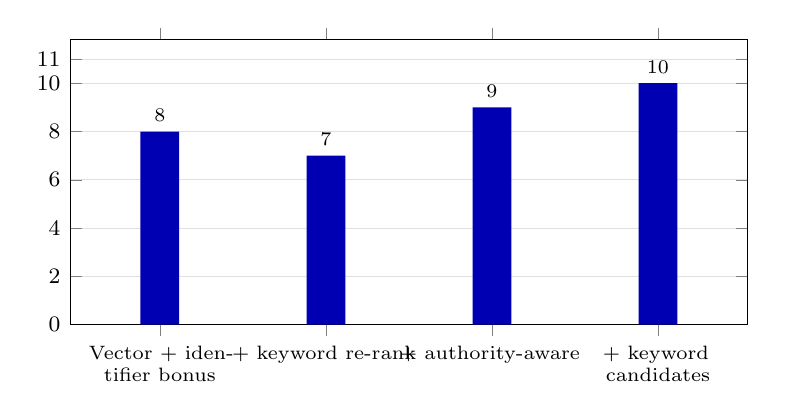
\begin{tikzpicture}
\begin{axis}[ybar,bar width=14pt,width=0.84\textwidth,height=5.2cm,
  symbolic x coords={V1,V2,V3,V4},xtick=data,
  xticklabels={Vector + identifier bonus,+ keyword re-rank,+ authority-aware,+ keyword candidates},
  x tick label style={font=\scriptsize,text width=2.5cm,align=center},
  ymin=0,ymax=11.8,ytick={0,2,4,6,8,10,11},ymajorgrids,grid style={black!12},
  tick label style={font=\footnotesize},nodes near coords,every node near coord/.append style={font=\scriptsize},
  enlarge x limits=0.18]
\addplot[fill=blue!70!black,draw=none] coordinates {(V1,8) (V2,7) (V3,9) (V4,10)};
\end{axis}
\end{tikzpicture}
\caption{Questions (of 11) whose expected document is in the top 3, by retrieval version. Keyword re-ranking alone lowered recall; authority-aware ranking and keyword-matched candidates raised it to 10 of 11.}\label{fig:retrabl}
\end{figure}

\subsection*{Finding 2: what the model is shown matters as much as what is retrieved}
\textbf{Claim.} A correct retrieval can still starve the model of the answer. \textbf{Evidence.} For the make-up deadline (Q03) and Minor-exam dates (Q06) the right chunks were retrieved and contained the facts (``ten days'', ``15--20 September 2026''), but the 1,000-character window sent to the model omitted them; facts present in the evidence were 22 of 25 before the fix and 24 of 25 after. \textbf{Interpretation.} The window had been chosen by raw word frequency, which common words (``exam'', ``semester'') dominate. Scoring windows by the IDF weight of the distinct query words, and giving the top passage up to 1.8 times the cap within the same total budget, fixed both cases without increasing request size.

\subsection*{Finding 3: deterministic tools make specialisation pay; the limit is the corpus}
\textbf{Claim.} Where an answer is computable, giving it to a tool removes the model from the failure path. \textbf{Evidence.} Timetable and email questions have complete evidence in 14 of 14 cases (Table~\ref{tab:evidence}) and 48 tool assertions pass, including the clash check for courses with no slot code. Policy questions reach 10 of 11, limited by Q11, which the corpus does not answer. \textbf{Interpretation.} Specialisation helps when each specialist has a small, exact toolset; whether the multi-agent split beats the single-agent baseline on answer accuracy is not established here, because the single-agent baseline was not evaluated.

\subsection*{Finding 4: request size, not computation, sets latency on a rate-limited tier}
\textbf{Claim.} Shorter prompts and fewer tools per agent reduce turn time. \textbf{Evidence.} Measured request sizes for one question fell from 1,788, 3,325 and 4,746 tokens on calls 1--3 to 1,386, 2,026 and 3,237 (plus a fourth call of 4,632 when the model searched twice); turn time for the attendance question fell from about 120~s to about 70~s (Table~\ref{tab:tokens}). \textbf{Interpretation.} A turn makes three to five model calls, each re-sending instructions, tool definitions and history, which exceeds the roughly 7,000-token-per-minute cap of the free tier even with no other load; the remaining time is waiting for the limit to refill.

\begin{table}[H]
\centering\small
\caption{Approximate request size per model call for one question (tokens, estimated at 3.6 characters per token).}\label{tab:tokens}
\begin{tabular}{@{}lcccc@{}}
\toprule
 & \textbf{Call 1} & \textbf{Call 2} & \textbf{Call 3} & \textbf{Call 4}\\
\midrule
Before trimming & 1,788 & 3,325 & 4,746 & --\\
After trimming & 1,386 & 2,026 & 3,237 & 4,632\\
\bottomrule
\end{tabular}
\end{table}

\begin{figure}[H]
\centering
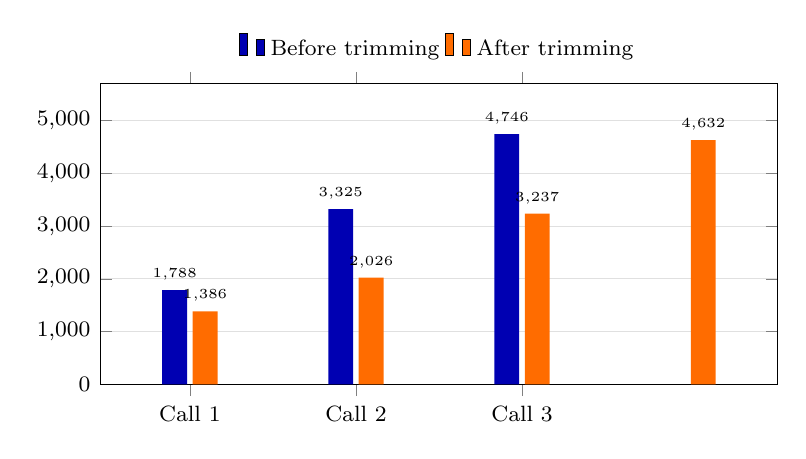
\begin{tikzpicture}
\begin{axis}[ybar,bar width=9pt,width=0.84\textwidth,height=5.4cm,
  symbolic x coords={C1,C2,C3,C4},xtick=data,xticklabels={Call 1,Call 2,Call 3,Call 4},
  ymin=0,ymax=5700,ytick={0,1000,2000,3000,4000,5000},ymajorgrids,grid style={black!12},
  tick label style={font=\footnotesize},
  legend style={at={(0.5,1.04)},anchor=south,legend columns=-1,font=\footnotesize,draw=none},
  nodes near coords,every node near coord/.append style={font=\tiny},enlarge x limits=0.18]
\addplot[fill=blue!70!black,draw=none] coordinates {(C1,1788) (C2,3325) (C3,4746)};
\addplot[fill=orange!85!red,draw=none] coordinates {(C1,1386) (C2,2026) (C3,3237) (C4,4632)};
\legend{Before trimming,After trimming}
\end{axis}
\end{tikzpicture}
\caption{Estimated request size (tokens) per model call for one question. Trimming lowered every call; the fourth call exists only after a second search.}\label{fig:tokbar}
\end{figure}

\subsection*{Finding 5: scope refusal cannot rest on retrieval alone}
\textbf{Claim.} A distance threshold does not separate in-scope from out-of-scope questions. \textbf{Evidence.} Best cosine distance is 0.28--0.62 for in-scope and 0.47--0.74 for out-of-scope questions, an overlap of 0.142. At the 0.50 threshold four of five out-of-scope questions fail the evidence check; Q27 (reaching the campus from the city) passes it. \textbf{Interpretation.} The orchestrator's explicit list of out-of-scope topics is the real safeguard, which makes refusal behaviour dependent on the model following its prompt. Its strength was observed on one question (dining); the correct-refusal rate over Q26--Q30 was not measured on the model.

\subsection*{Finding 6: model comparison is not established}
\textbf{Claim.} Which of the two models is better, whether either is unsuitable, and which answers change between repetitions cannot be stated. \textbf{Evidence.} No model-answer score was completed (Table~\ref{tab:status}). \textbf{Interpretation.} The comparison the project plan calls for remains open; the point estimates in Section~\ref{sec:estimates} are illustrative assumptions and not comparative evidence; the harness and the commands that produce measured results are in Section~\ref{sec:repro}. A third model, \code{llama-3.1-8b-instant}, was planned but is no longer served by the provider (the API returned \code{model_not_found}).

% =====================================================================
\section{Failure Modes and Limitations}\label{sec:limits}
% =====================================================================
\begin{enumerate}
  \item \textbf{Scope refusal depends on the prompt.} Q27 has best distance 0.479 and passes the evidence check; only the orchestrator's scope list refuses it.
  \item \textbf{Conflicting sources.} The 2019 and 2022 regulations and the July 2024 amendment give different attendance rules. Authority-aware ranking addresses retrieval, but after the prompts were shortened the policy agent still hedged on this question once (Section~\ref{sec:results}).
  \item \textbf{Information absent from the corpus.} Q11 (Open Elective credits for B.Tech.) has no stated total: the curricula combine Programme and Open Electives (for CSE, 6 + 15 credits in the last two semesters of 150 graded credits). The expected document ranks 10th.
  \item \textbf{Structured-data provenance.} Which rows of \code{courses.csv} and \code{faculty.csv} are verified is unrecorded; office contact addresses and the Cc line are placeholders.
  \item \textbf{Small evaluation set.} With 30 questions, one question is 3.3 percentage points overall and 9.1 points within the 11 policy questions; differences of a few points between configurations may be noise. Two configurations with 2--3 repetitions do not support strong claims.
  \item \textbf{Latency.} About 70~s per turn on the free tier when the account is otherwise idle; under the evaluation load the runs were held back by waits of 76 to 90 seconds. Per-question latency was not recorded, so accuracy cannot be related to latency; only the turn time of one question before and after trimming was measured.
  \item \textbf{Strict scoring.} Groundedness requires an expected source identifier in the answer; an answer that names a document in words only scores as ungrounded. Correct answers were initially marked wrong when the model used non-breaking spaces or curly quotes; scoring now normalises text, but residual mismatches remain possible.
  \item \textbf{Ground-truth errors.} Q18 originally expected 8 courses in slot G; one was from Semester II 2025--26, so the correct current-semester count is 7. An error in the reference answers would silently penalise a correct system.
  \item \textbf{Incomplete model evaluation.} Model-answer metrics, the single-agent baseline and a cross-model comparison were not completed (Section~\ref{sec:results}); Section~\ref{sec:estimates} gives illustrative point estimates only.
  \item \textbf{Native-library instability.} ChromaDB's native index crashed and ONNX Runtime 1.22 or later failed to initialise on the development machine; the system therefore pins ONNX Runtime 1.20.1 and offers an exact NumPy search.
  \item \textbf{Exposed credential.} The API key was committed early and remains in repository history.
  \item \textbf{Local deployment untested.} The assignment suggests an 8B model served by Ollama and a local embedding model on a 16~GB machine. The system supports this by changing one configuration string, but no local-model run was made, so the 16~GB requirement and the quality of an 8B model are unverified; all model behaviour reported here is from hosted models.
\end{enumerate}

% =====================================================================
\section{Recommendations and Future Work}\label{sec:future}
% =====================================================================
\begin{enumerate}
  \item Complete the model evaluation and report the single-agent baseline, so the value of delegation can be stated (limitations 5, 9).
  \item Add a deterministic scope classifier in front of the orchestrator for the listed out-of-scope topics, so refusal no longer depends on the prompt alone (limitation 1).
  \item Re-run the attendance question and the other policy questions after the refusal-rule change, and add a regression test for ``rule relaxed by an amendment'' (limitation 2).
  \item Add an exam-schedule table to the structured data so dates need not be retrieved from calendar text, and ask a human to confirm Q11's answer with the Academic Office (limitations 3, 4).
  \item Record per-row provenance and a \code{verified} column for every structured file, and replace placeholder contact addresses with verified ones (limitation 4).
  \item Record latency and token use per question in the evaluation harness so accuracy-versus-latency can be reported (limitation 6).
  \item Reduce per-turn calls by returning compact tool results and caching agent prefixes where the provider allows (limitation 6).
  \item Review every reference answer against its source before scoring, and have a second person check them (limitation 8).
  \item Rotate the exposed API key and keep keys out of version control (limitation 11).
  \item Run the evaluation once with a local 8B model through Ollama on a 16~GB machine, to confirm the deployment requirement and to compare a small local model with the hosted ones (limitation 12).
\end{enumerate}

% =====================================================================
\section{Reproducibility}\label{sec:repro}
% =====================================================================
\textbf{Setup.}
\begin{lstlisting}[language=bash]
git clone https://github.com/Sharan4405/Academic-_Helpdesk_Agent.git
cd Academic-_Helpdesk_Agent
python -m venv .venv
.\.venv\Scripts\Activate.ps1
pip install -r requirements.txt
Copy-Item .env.example .env          # then set GROQ_API_KEY in .env
python -m academic_helpdesk.rag.import_prebuilt
\end{lstlisting}
\textbf{Verification and evaluation.}
\begin{lstlisting}[language=bash]
python eval/check_tools.py           # 48 deterministic assertions
python eval/check_retrieval.py       # recall and refusal separability
python eval/evidence_eval.py         # evidence evaluation, all 30 questions
python eval/run_eval.py --runs 3 --mode multi --tag qwen27-multi
python eval/run_eval.py --runs 2 --mode multi --model groq/openai/gpt-oss-20b --tag gptoss20-multi
python eval/make_report_assets.py    # tables (CSV/JSON) and charts for the model runs
\end{lstlisting}
\textbf{Interactive use.}
\begin{lstlisting}[language=bash]
python -m academic_helpdesk.cli --trace                  # terminal client
python -m academic_helpdesk.cli --mode single            # single-agent baseline
python -m web.backend.service                            # web demo, http://127.0.0.1:8000
\end{lstlisting}

% =====================================================================
\section{Conclusion}
% =====================================================================
The helpdesk shows that a question-answering assistant can be made trustworthy by moving everything computable out of the model and making refusal depend on evidence. Counts, slots and contacts come from tools; rules come from retrieval that knows which circular supersedes which; drafts are rendered from fixed templates; a terminal client and a web interface expose the same system. Without a chat model, the evidence handed to the agent is right for 24 of 25 answerable questions, and the expected document ranks first for 10 of 11 policy questions. The pattern that emerged is that the weak points were in the evidence and the prompts, not in retrieval recall. The best configuration and its trade-off against latency cannot yet be stated, because no scored model run was completed; the point estimates in Section~\ref{sec:estimates} are illustrative assumptions, not findings.

The single most important engineering lesson is to read what the model is actually given. Two of the defects found---a passage window that cut off the answer, and a reference answer that counted a past-semester course---looked like model errors until the inputs were inspected.

% =====================================================================
\appendix
\section{Evaluation Questions}
% =====================================================================
\begin{longtable}{@{}>{\ttfamily}l p{0.84\textwidth}@{}}
\caption{The 30 evaluation questions (category in parentheses).}\\
\toprule
\textbf{ID} & \textbf{Question}\\
\midrule
\endfirsthead
\toprule
\textbf{ID} & \textbf{Question}\\
\midrule
\endhead
Q01 & What is the attendance requirement to sit in the Major exam? \textit{(rules)}\\
Q02 & How many examinations are held in a semester and how long is the Major exam? \textit{(rules)}\\
Q03 & By when must I apply for a make-up exam if I miss the Major exam because of illness? \textit{(rules)}\\
Q04 & Until when can I withdraw from a course, and how does it appear on my grade card? \textit{(rules)}\\
Q05 & What is the last date to add or drop courses in Semester I of 2026-27? \textit{(rules)}\\
Q06 & When is the Minor examination in Semester I of 2026-27? \textit{(rules)}\\
Q07 & How many credits is one hour of lab per week worth, compared with one hour of lecture? \textit{(rules)}\\
Q08 & When is an undergraduate student placed on academic probation? \textit{(rules)}\\
Q09 & How can I convert my CGPA into a percentage? \textit{(rules)}\\
Q10 & What is the semester fee for a hosteller in Academic Year 2026-27? \textit{(rules)}\\
Q11 & How many Open Elective credits do I need to earn in order to get a B.Tech. degree? \textit{(rules)}\\
Q12 & What is the slot for the course Autonomous Systems? \textit{(timetable)}\\
Q13 & How many 400 level electives have been floated by the Humanities department in this semester? \textit{(timetable)}\\
Q14 & Who teaches CSL7570 and in which slot does it meet? \textit{(timetable)}\\
Q15 & How many 400 level courses has the Computer Science and Engineering department floated this semester? \textit{(timetable)}\\
Q16 & Can I register for both HSL4010 and HSL4070 in the same semester, or do their slots clash? \textit{(timetable)}\\
Q17 & What are the days and timings of slot A? \textit{(timetable)}\\
Q18 & How many courses are scheduled in slot G this semester? \textit{(timetable)}\\
Q19 & How many credits is Computational Game Theory, and which room is it in? \textit{(timetable)}\\
Q20 & How many Electrical Engineering courses are offered this semester? \textit{(timetable)}\\
Q21 & Write an email to the course instructor of CSL7570 that I need leave for 2 days. \textit{(email)}\\
Q22 & I was ill and missed the CSL4100 Major exam on 20 November 2026. Draft an email to the instructor asking for a make-up exam. \textit{(email)}\\
Q23 & My attendance in IDL4010 is 68\%. Write an email to the instructor requesting attendance condonation. \textit{(email)}\\
Q24 & Draft a sick leave email to the HSL4010 instructor for 3 August 2026 to 5 August 2026. \textit{(email)}\\
Q25 & What is the email address of the instructor of ECL4010? \textit{(email)}\\
Q26 & What are the available dining options on the campus? \textit{(out of scope)}\\
Q27 & What is the best way to reach the campus from Jodhpur city center? \textit{(out of scope)}\\
Q28 & What is the weather in Jodhpur today? \textit{(out of scope)}\\
Q29 & What is my current attendance in CSL4100? \textit{(out of scope)}\\
Q30 & What are the opening hours of the gym and swimming pool on campus? \textit{(out of scope)}\\
\bottomrule
\end{longtable}

\section{References}
\begin{enumerate}[label={[\arabic*]}]
  \item Project repository: \url{https://github.com/Sharan4405/Academic-_Helpdesk_Agent}
  \item Google Agent Development Kit documentation: \url{https://google.github.io/adk-docs/}
  \item LiteLLM documentation: \url{https://docs.litellm.ai/}
  \item ChromaDB documentation: \url{https://docs.trychroma.com/}
  \item all-MiniLM-L6-v2 sentence-embedding model: \href{https://huggingface.co/sentence-transformers/all-MiniLM-L6-v2}{Hugging Face model card}
  \item Groq API documentation: \url{https://console.groq.com/docs}
  \item IIT Jodhpur Office of Academic Affairs: \url{https://iitj.ac.in/office-of-academics/}
  \item Source documents: the 29 URLs recorded in \code{data1/manifest_source.csv}.
\end{enumerate}

\end{document}